%%%%%%%%%%%%%%%%%%%%%%%%%%%%%%%%%%%%%%%%%
% Masters/Doctoral Thesis 
% LaTeX Template
% Version 2.2 (21/11/15)
%
% This template has been downloaded from:
% http://www.LaTeXTemplates.com
%
% Version 2.x major modifications by:
% Vel (vel@latextemplates.com)
%
% This template is based on a template by:
% Steve Gunn (http://users.ecs.soton.ac.uk/srg/softwaretools/document/templates/)
% Sunil Patel (http://www.sunilpatel.co.uk/thesis-template/)
%
% Template license:
% CC BY-NC-SA 3.0 (http://creativecommons.org/licenses/by-nc-sa/3.0/)
%
%%%%%%%%%%%%%%%%%%%%%%%%%%%%%%%%%%%%%%%%%

%----------------------------------------------------------------------------------------
%	PACKAGES AND OTHER DOCUMENT CONFIGURATIONS
%----------------------------------------------------------------------------------------

\documentclass[
11pt, % The default document font size, options: 10pt, 11pt, 12pt
oneside, % Two side (alternating margins) for binding by default, uncomment to switch to one side
english, % ngerman for German
singlespacing, % Single line spacing, alternatives: onehalfspacing or doublespacing
%draft, % Uncomment to enable draft mode (no pictures, no links, overfull hboxes indicated)
%nolistspacing, % If the document is onehalfspacing or doublespacing, uncomment this to set spacing in lists to single
%liststotoc, % Uncomment to add the list of figures/tables/etc to the table of contents
%toctotoc, % Uncomment to add the main table of contents to the table of contents
%parskip, % Uncomment to add space between paragraphs
%nohyperref, % Uncomment to not load the hyperref package
headsepline, % Uncomment to get a line under the header
]{MastersDoctoralThesis} % The class file specifying the document structure

\usepackage[utf8]{inputenc} % Required for inputting international characters
\usepackage[T1]{fontenc} % Output font encoding for international characters
\usepackage{amsmath,amssymb}
\usepackage{algorithm}
\usepackage{algpseudocode}


\usepackage{palatino} % Use the Palatino font by default
\usepackage{float} %force position of figures
\usepackage{wrapfig} %for wrapping images
\usepackage{longtable} %for creating tables across several pages
\usepackage{tabu} %for creating long tables
\usepackage{booktabs}
\usepackage{lscape}
\usepackage{seqsplit}
\usepackage{graphicx}
\usepackage[table,xcdraw]{xcolor}
\usepackage{cleveref}
\usepackage{adjustbox}



\usepackage[backend=bibtex,style=ieee,maxcitenames=3,natbib=true]{biblatex} % User the bibtex backend with the authoryear citation style (which resembles APA)
\addbibresource{kilder.bib} % The filename of the bibliography

\usepackage[autostyle=true]{csquotes} % Required to generate language-dependent quotes in the bibliography

\usepackage[xindy={language=german,codepage=duden-utf8}, acronym, toc]{glossaries}
\usepackage{todonotes}

%%CUSTOM USE PACKAGES NOT FROM TEMPLATE
\usepackage{enumitem} %% USED FOR NO SPACE BETWEEN BULLET POINTS (DESIGN SECTION)
\usepackage{scrextend}
\usepackage{tabto}

\usepackage{verbatim}

\usepackage{titlesec}

\titleformat{\chapter}{\normalfont\huge}{\thechapter.}{20pt}{\huge\bf}

\nocite{*}

%%USED TO DISPLAY CODE

\definecolor{pblue}{rgb}{0.13,0.13,1}
\definecolor{pgreen}{rgb}{0,0.5,0}
\definecolor{pred}{rgb}{0.9,0,0}
\definecolor{pgrey}{rgb}{0.46,0.45,0.48}
\definecolor{lightb}{RGB}{217,224,250}
\definecolor{SDUblue}{RGB}{1,67,128}

\usepackage{listings}
\lstset{language=Java,
  showspaces=false,
  showtabs=false,
  breaklines=true,
  showstringspaces=false,
  breakatwhitespace=true,
  commentstyle=\color{pgreen},
  keywordstyle=\color{pblue},
  stringstyle=\color{pred},
  basicstyle=\ttfamily,
  moredelim=[il][\textcolor{pgrey}],
  moredelim=[is][\textcolor{pgrey}]{\%\%}{\%\%}
}


\makeglossaries
	
%!TEX root=../main.tex

%%%%%%%%%%% GLOSSARY ENTRIES %%%%%%%%%%%
\newglossaryentry{NoSQL}
{
	name=\textit{No-SQL},
	plural=\textit{No-SQL},
	description={Not Only SQL: a database which relies on collections and documents rather than the classical relational databases with tables, columns and rows}
}

\newglossaryentry{Struct}
{
	name=\textit{Struct A/S},
	plural=\textit{Struct A/S},
	description={A company specializing in E-commerce solutions for businesses Struct has partnered with the project group and supplied the data for this Bachelor project}
}

\newglossaryentry{MongoDB}
{
	name=\textit{MongoDB},
	plural=\textit{MongoDB},
	description={A No-SQL database implementation}
}

\newglossaryentry{Amazon}
{
	name=\textit{Amazon},
	plural=\textit{Amazon},
	description={Amazon is a retail giant selling product to consumers in many different categories}
}

\newglossaryentry{EC2Instance}
{
	name=\textit{EC2 Instance},
	plural=\textit{EC2 Instances},
	description={A linux based virtual server running in the AWS cloud}
}

\newglossaryentry{ecommerce}
{
	name=\textit{e-commerce},
	plural=\textit{e-commerces},
	description={The business of buying and selling online}
}

\newglossaryentry{datamining}
{
	name=\textit{datamining},
	description={An analysis technique trying to discover useful information and relationships in large amounts of existing data}
}

\newglossaryentry{gls-API}
{
	name=\textit{API},
	description={An interface designed to integrate one piece of software with another}
}

\newglossaryentry{contentbased}
{
	name=\textit{Content-based filtering},
	description={A recommendation technique focusing on the content (description) of an item and how it relates to other items}
}

\newglossaryentry{knowledgebased}
{
	name=\textit{Knowledge-based recommendations},
	description={A recommendation technique relying on deep knowledge about the offered items}
}

\newglossaryentry{collaborativefiltering}
{
	name=\textit{Collaborative filtering},
	description={A recommendation technique linking items and users based on user-behavior, item descriptions etc.}
}

\newglossaryentry{hybrid}
{
	name=\textit{Hybrid recommendations},
	description={A mix of other recommendation techniques such is \gls{contentbased}, \gls{knowledgebased} and \gls{collaborativefiltering}}
}

\newglossaryentry{aspnet}
{
	name=\textit{ASP.NET Core},
	description={Open-source and cross-platform framework for building modern internet connected applications. It consists of modular components with minimal overhead to retain flexibility when constructing solutions}
}

\newglossaryentry{gls-REST}
{
	name=\textit{REST},
	description={An architectural style used for communication across systems on the internet}
}

\newglossaryentry{Docker}
{
	name=\textit{Docker},
	description={Docker is an open-source project that automates the deployment of applications inside software containers}
}

\newglossaryentry{amazonwebservice}
{
	name=\textit{Amazon Web-services},
	description={Provides on-demand cloud computing platforms}
}

\newglossaryentry{DockerContainer}
{
	name=\textit{Docker container},
	description={A lightweight stand-alone executable package of a piece of software that includes everything needed to run it}
}




%%%%%%%%%%% ACRONYMS %%%%%%%%%%%

\newacronym{DTO}{\textit{DTO}}{Data transfer object}

\newacronym[see={[Glossary:]{gls-API}}]{API}{\textit{API}}{Application Programming Interface\glsadd{gls-API}}

\newacronym[see={[Glossary:]{gls-REST}}]{REST}{\textit{REST}}{REpresentational State Transfer\glsadd{gls-REST}}

\newacronym{HTTP}{\textit{HTTP}}{HyperText Transfer Protocol}

\newacronym{XML}{\textit{XML}}{Extensible Markup Language}




%----------------------------------------------------------------------------------------
%	MARGIN SETTINGS
%----------------------------------------------------------------------------------------

\geometry{
	paper=a4paper, % Change to letterpaper for US letter
	inner=1.5cm, % Inner margin
	outer=1.5cm, % Outer margin
	bindingoffset=1cm, % Binding offset
	top=1.5cm, % Top margin
	bottom=1.5cm, % Bottom margin
	%showframe,% show how the type block is set on the page
}

%----------------------------------------------------------------------------------------
%	THESIS INFORMATION
%----------------------------------------------------------------------------------------

\thesistitle{Datamining and its use} % Your thesis title, this is used in the title and abstract, print it elsewhere with \ttitle
\supervisor{Jan Corfixen Sørensen} % Your supervisor's name, this is used in the title page, print it elsewhere with \supname
\examiner{} % Your examiner's name, this is not currently used anywhere in the template, print it elsewhere with \examname
\degree{Software Engineering Bachelor Project $6^{th}$  semester} % Your degree name, this is used in the title page and abstract, print it elsewhere with \degreename
\author{Lasse Bjørn Hansen\\
		Simon Flensted \\
		\textit{\small lahan14@student.sdu.dk\\
		sifle14@student.sdu.dk}} % Your name, this is used in the title page and abstract, print it elsewhere with \authorname
\addresses{} % Your address, this is not currently used anywhere in the template, print it elsewhere with \addressname

\subject{Software Engineering} % Your subject area, this is not currently used anywhere in the template, print it elsewhere with \subjectname
\keywords{} % Keywords for your thesis, this is not currently used anywhere in the template, print it elsewhere with \keywordnames
\university{University of Southern Denmark} % Your university's name and URL, this is used in the title page and abstract, print it elsewhere with \univname
\department{TEK} % Your department's name and URL, this is used in the title page and abstract, print it elsewhere with \deptname
\group{Group ??} % Your research group's name and URL, this is used in the title page, print it elsewhere with \groupname
\faculty{TEK - Mærsk McKinney Møller Institut} % Your faculty's name and URL, this is used in the title page and abstract, print it elsewhere with \facname

\hypersetup{pdftitle=\ttitle} % Set the PDF's title to your title
\hypersetup{pdfauthor=\authorname} % Set the PDF's author to your name
\hypersetup{pdfkeywords=\keywordnames} % Set the PDF's keywords to your keywords

\begin{document}

\frontmatter % Use roman page numbering style (i, ii, iii, iv...) for the pre-content pages

\pagestyle{plain} % Default to the plain heading style until the thesis style is called for the body content

%----------------------------------------------------------------------------------------
%	TITLE PAGE
%----------------------------------------------------------------------------------------

\begin{titlepage}
\begin{center}

\textsc{\LARGE \univname}\\[1.5cm] % University name
\textsc{\Large \degreename}\\[0.5cm] % Thesis type

\HRule \\[0.4cm] % Horizontal line
{\huge \bfseries \ttitle}\\[0.4cm] % Thesis title
\HRule \\[1.5cm] % Horizontal line
 
\begin{minipage}{0.4\textwidth}
\begin{flushleft} \large
\emph{Author:}\\
\authorname % Author name - remove the \href bracket to remove the link
\end{flushleft}
\end{minipage}
\begin{minipage}{0.4\textwidth}
\begin{flushright} \large
\emph{Supervisor:} \\
{\supname} % Supervisor name - remove the \href bracket to remove the link  
\end{flushright}
\end{minipage}\\[3cm]

\includegraphics{SDU-Logo}\\ % University/department logo - uncomment to place it
\large \textit{A report submitted in fulfillment of the requirements\\  of \degreename}\\[0.3cm] % University requirement text
\textit{at}\\[0.4cm]
\univname\\\facname\\[2cm] % Research group name and department name
 
{\large \today}\\[4cm] % Date

 
\vfill
\end{center}
\end{titlepage}

%----------------------------------------------------------------------------------------
%	ABSTRACT PAGE
%----------------------------------------------------------------------------------------

\thispagestyle{plain}

\chapter{Abstract}
\textit{Datamining has become a growing part of modern software solutions. In the business of e-commerce, companies have realized how important prober analysis and organization of data can be to increase sales. Once data is organized in a desirable manner, companies can exploit the data to learn more about their customers.\\
This paper describes the initial datamining of a large datadump, a system for maintaining the data and an algorithm that provides tailored product recommendations to visitors of a webshop.
The development of the algorithm is inspired by similar existing systems, among these the retail giant Amazon. The final product is designed according to the requirements acquired from the collaborating company Struct A/S.}
\clearpage

%----------------------------------------------------------------------------------------
%	PREFACE / ACKNOWLEDGMENTS
%----------------------------------------------------------------------------------------

\chapter{Preface}
This report has been written by Lasse Bjørn Hansen and Simon Haugaard Flensted. It is the documented result of a bachelor project at the 6th semester of Software Engineering at University of Southern
Denmark in Odense (01/02/2017 - 22/05/2017). The report documents the implementation and the final product of the project.\\

\noindent We would like to thank our bachelor supervisor Jan Corfixen Sørensen for guiding, being available and helping throughout the project. We would also like to thank the company \gls{Struct}, especially Peter Melchiorsen and Simon Lyder for providing the case that formed the foundation of the project, and providing continuous feedback. At last the group would like to thank Casper Middelhede and Lars Bo Meixner for reading through this report and providing valuable feedback.
\\

\noindent This report was handed in May 22, 2017.
\\
\\
\\

\noindent\rule[0.5em]{26em}{0.5pt}\\
\noindent Lasse Bjørn Hansen \tab 64753953
\\
\\

\noindent\rule[0.5em]{26em}{0.5pt}\\
\noindent Simon Haugaard Flensted \tab 409994
\\
\\

%----------------------------------------------------------------------------------------
%	QUOTATION PAGE
%----------------------------------------------------------------------------------------

\vspace*{0.2\textheight}

\noindent\Large{\enquote{\itshape We think the combined effect of personalization
and recommendations save us more than \$1B per year}}\bigbreak
\hfill \large{- Neil Hunt, Netflix's Chief Product Officer}
\normalsize

%----------------------------------------------------------------------------------------
%	READING GUIDE
%----------------------------------------------------------------------------------------

\thispagestyle{plain}
% Chapter Template

\chapter{Reading guide} % Main chapter title

\label{readingGuide} % Change X to a consecutive number; for referencing this chapter elsewhere, use \ref{ChapterX}

%----------------------------------------------------------------------------------------
%	SECTION 1
%----------------------------------------------------------------------------------------

This report is targeted at readers with similar knowledge as a student on the 6th semester of
Software Engineering. The report
is divided into 10 main chapters, each split into sections and subsections depending on the content.
Each chapter can be read separately, but it is recommended to read the report in chronological order
to achieve the best possible insight into the project. The report does not contain a profound theoretical
description of the implementation, but explains the final product as it is implemented. It is
recommended to study theoretical parts if the reader is not familiar with used terms.
Chapter one introduces the motivation behind the project, key areas, and an introduction of the company collaborated with. Chapter two describes the problem description and problem statement. Chapter three describe the
requirements of the product and their role throughout the project. Chapter four contains an analysis
of the requirements and presents the domain. Chapter five introduces the design of the
product while Chapter six describes the implementation. In chapter seven validation of the code and validation of the recommendations are provided. Chapter eight discusses how well the system was implemented and what other solution might have been possible. Chapter nine concludes the project and answers the problem statement. Chapter ten discuss further development of the product and the benefits hereof.\\
All figures in this report will be referenced to as "figure X.Y" where X corresponds to the chapter in
which the figure can be found and Y corresponds to the number of the figure. Figure 4.4 would as an
example refer to figure 4 in Chapter 4. Each figure will include a caption that describes the individual
figures. Chapters and appendices will be referenced as "chapter 4" or "Appendix A". Appendices are found in the back of the report.
All source references are noted with brackets [1], as stated in the IEEE Citation Reference [ieee]. The number
corresponds to the assigned place in the bibliography. All books, websites, articles etc. used can be
found in the Bibliography section at the end of this report.
%----------------------------------------------------------------------------------------
%	LIST OF CONTENTS/FIGURES/TABLES PAGES
%----------------------------------------------------------------------------------------

\setcounter{tocdepth}{1}
\tableofcontents % Prints the main table of contents
\clearpage

%----------------------------------------------------------------------------------------
%	EDITORIAL
%----------------------------------------------------------------------------------------

%\thispagestyle{plain}


%----------------------------------------------------------------------------------------
%	GLOSSARY LIST
%----------------------------------------------------------------------------------------

\printglossaries

%----------------------------------------------------------------------------------------
%	THESIS CONTENT - CHAPTERS
%----------------------------------------------------------------------------------------

\mainmatter % Begin numeric (1,2,3...) page numbering

\pagestyle{thesis} % Return the page headers back to the "thesis" style

% Include the chapters of the thesis as separate files from the Chapters folder
% Uncomment the lines as you write the chapters
% Chapter Template

\chapter{Introduction} % Main chapter title

\label{ChapterX} % Change X to a consecutive number; for referencing this chapter elsewhere, use \ref{ChapterX}

%----------------------------------------------------------------------------------------
%	SECTION 1
%----------------------------------------------------------------------------------------

This chapter covers the motivation behind the project and important areas relating to the project. It introduces the collaborating company who helped provide a case, data, and feedback. Finally the scope of the project is defined.

\section{Motivation}
The amount of data being processed on the server side and within large systems is continuously increasing. This data should be structured and modeled in a way that makes it easily accessible and easy to work with. Handling large amounts of data the right way can prove to be very useful, not only to the company who possesses the data, but also to the end users of a product. \Gls{datamining} is very useful in order to achieve this.
The company Struct A/S has provided a software engineering task of creating product recommendations where data mining will create the foundation. This report will address the use of data mining, the development of a solution that provides the user with intelligent product recommendations, and makes it possible to maintain current and future data.

\subsection{Data mining}
Data mining is an analysis technique trying to discover useful information and relationships in large amounts of existing data \cite{dataminingSource}. \\  
Data mining has become an important part of modern software engineering. Lots of companies tends to store large amount of data. If the data is analyzed properly and put to use, it can add tremendous value to the company as well as its users. In this case \gls{Struct} has stored information about users visiting one of their customers webshops. Previously, this data was stored in a database not optimized for product recommendations and not put to use. By processing the data properly, using data mining, it can be structured in a way that makes it useful to the company e.g. product recommendations.

\color{black}
\subsection{Product recommendation}
If an e-commerce company wants to increase its profit, product recommendation has proven to be very beneficial \cite{BigCommerce}. This is heavily used by multiple companies including the retail giant Amazon\cite{Fortune}. If you can predict what products your costumer may find useful, additional sales become more frequent. A data set like the one provided by Struct A/S, can make it possible to predict customer needs.

\section{Struct A/S}
Struct A/S is an IT-company specializing in developing E-commerce solutions such as web shops and Product Information Management systems. The customers of Struct A/S are the web shop owners. Struct A/S has provided a data set from one of these customers containing information about the visitors of their web shop \cite{Struct}.


\section{Scope}
Product recommendation and data mining are massive subjects consisting of much literature. Many large companies have tackled the challenge of providing recommendations for their users and spent a lot of time perfecting their algorithms.\\
This project will focus on designing and implementing a product recommendation algorithm capable of providing "good recommendations" The term "good recommendations" is a very loose term because it can vary from business to business or even from individual to individual. To directly compare the developed algorithm to others on the market would require access to these algorithms as well as a test on the same data. This has not been possible to acquire and therefore no direct comparison will be made. \\
In the limited time of this project it is not reasonable to expect Struct A/S to be able to begin using the API which means no online validation can be made. \\
The project comes with limited funds and as a result of this, some less optimal but free alternatives have been used for hosting the algorithm. \\
Only the requirements necessary to have a functional product are implemented as there is ample material to focus on.

% Chapter Template

\chapter{Problem statement} % Main chapter title

\label{Chapter1} % Change X to a consecutive number; for referencing this chapter elsewhere, use \ref{ChapterX}

%----------------------------------------------------------------------------------------
%	SECTION 1
%----------------------------------------------------------------------------------------

\section{Problem description}

The initial problem/challenge  is given to us by the company Struct A/S and is described as follows: \\\\
When launching sites, whether it being regular websites or web shops, a lot of user activity is logged. We therefore have a large amount of data associated with each of our sites but do not currently use it. \\
In the future we would like to be able to use logged data to generate an insight into the user activity on our site and actively use this data to create a personalized experience for the users. \\\\

This project will handle the initial normalization of the data, storing it in a scalable way and utilizing the data to create features which add value for the users. In order to achieve this, theory has to become implementation. Research is required in terms of data storing, data mining and recommendation algorithms. This research is implemented in the end system creating an API allowing Struct A/S to get useful information from the data such as the recommended products for a certain user. This API will be the final product and will utilize different technologies and algorithms.





\section{Problem statement}
The data we have been given is in a de-normalized format and the problem therefore comes with two challenges - normalizing the data and utilizing the data to create a personalized experience for the users. \\
This leads to the following research questions:
\begin{itemize}
\item How can you effectively normalize large amounts of data?
\item How can you optimally store and access data in a scalable way?
\item How can you utilize the data to generate useful features for the end user?
\end{itemize}

% Chapter Template

\chapter{Related work} % Main chapter title

\label{Chapter3} % Change X to a consecutive number; for referencing this chapter elsewhere, use \ref{ChapterX}

%----------------------------------------------------------------------------------------
%	SECTION 1
%----------------------------------------------------------------------------------------
This chapter different product recommendation approaches and state of the art as it relates to product recommendations. Amazon is also introduced as they are a big player in the product recommendation world.

\section{State of the art}

Datamining, web shop development and product recommendation algorithms are established parts of e-commerce development. This has resulted in great inspiration sources. In order to achieve the best possible result, some of the most successful developers of recommendation algorithms were researched. The video streaming service, Netflix, has invested a lot of resources in coming up with the best possible recommendation algorithm \cite{Netflix}. This includes a worldwide competition for \$1 million, called the Netflix Prize \cite{NetflixPrize}. Netflix can definitively be considered state of the art in the video streaming field. The retail giant, Amazon, is another company having great success with its product recommendation system. Amazon's product recommendation system plays a big part in increasing their sales \cite{AmazonSuccess}. What these two giants have in common, is that they are both using a collaborative recommendation algorithm. This is also the reason why the recommendation algorithm of this project is developed with the same technique, and will be elaborated further in chapter \ref{Chapter5}. Other techniques include content-based filtering, knowledge-based recommendations and hybrid recommendations. These techniques could be applied to the product, however, Content-based filtering is a good technique when recommending websites or articles. Knowledge-based recommendations is best put to use when high-involvement items are involved, such as cars, apartments, and financial services. Collaborative filtering best serves the purpose of product recommendations, due to its linking between users and items. Hybrid recommendations is a mix of all three methods \cite{recommendationtechniques}.


\section{Amazon}
Amazon has achieved great success with their recommendation system. There are many different techniques to develop a good product recommendation algorithm, but to develop one that is both smart, efficient and increases sale can be a difficult task. Some of the most common methods are user-to-user collaborative filtering, clustering and item-to-item collaborative filtering. Amazon's recommendation system is based on the latter, due to its fast pace response and precise recommendations. When developing a user-to-user collaborative filtering algorithm the result is often a precise, but slow recommendation system. By developing a clustering system, the response time can be very fast, but the quality of the recommendation will not be good \cite{AmazonRecommendations}. Other recommendation systems have been developed, but Amazon comes out as one of the greatest successors in the business and their recommendation system is one of their strong assets \cite{AmazonSuccess2}.

% Chapter Template

\chapter{Requirements} % Main chapter title

\label{Chapter3} % Change X to a consecutive number; for referencing this chapter elsewhere, use \ref{ChapterX}

%----------------------------------------------------------------------------------------
%	SECTION 1
%----------------------------------------------------------------------------------------

\section{Requirements engineering}
The requirements of the project are categorized into functional and non-functional requirements. These requirements were derived from the original case given by Struct A/S (Appendix \ref{Case}), continuously planned meetings with Struct A/S and our supervisor, and as a part of the constant research done during the progress of the project. \\
The functionality of the final product fulfills the most important aspects of the case, and the requirements derived from the client meetings.

\subsection{Functional requirements} 
The most important features of the system includes delivery of good quality product recommendation and handling of new data. These are very complex features and a lot of requirements must be fulfilled in order to realize them. The most crucial functional requirements can be seen in table \ref{table:functionalrequirements}. These requirements have been the driving force throughout the project. For a complete list of functional requirements, see the git backlog \cite{ProductBacklog}.
\begin{table}[]
	\centering
		\begin{tabular}{l|l}
			\rowcolor[HTML]{96B1FF} 
			\multicolumn{1}{c|}{\cellcolor[HTML]{96B1FF}F01} & \begin{tabular}[c]{p{.9\textwidth}}\textbf{The webshop developer can provide tailored product recommendations to his customers.}\\ When the API is provided with information about a visitor, tailored recommendations to the customer must be returned. If the data about the visitor is insufficient to calculate enough tailored recommendations, the most popular products within the last 30 days must be used to present enough recommendations.\end{tabular} \\
			F02                                              & \begin{tabular}[c]{p{.9\textwidth}}\textbf{The webshop developer can store new behavior data for a visitor in the database.} \\ When the API is provided with the required information, new behavior data must be stored in the database.\end{tabular}                                                                                                                                                                                                              \\
			\rowcolor[HTML]{96B1FF} 
			F03                                              & \begin{tabular}[c]{p{.9\textwidth}}\textbf{The webshop developer can store new behavior data for a product in the database.} \\ When the API is provided with the required information, new behavior data must be stored in the database.\end{tabular}                                                                                                                                                                                                              \\
			F04                                              & \begin{tabular}[c]{p{.9\textwidth}}\textbf{The webshop developer can store new product groups in the database.} \\ When the API is provided with the required information, a new product group must be stored in the database.\end{tabular}                                                                                                                                                                                                                         \\
			\rowcolor[HTML]{96B1FF} 
			F05                                              & \begin{tabular}[c]{p{.9\textwidth}}\textbf{The webshop developer can store new visitors in the database.}\\ When the API is provided with the required information, a new visitor must be stored in the database.\end{tabular}                                                                                                                                                                                                                                      \\
			F06                                              & \begin{tabular}[c]{p{.9\textwidth}}\textbf{The webshop developer can store new products in the database.}\\ When the API is provided with the required information, a new product must be stored in the database.\end{tabular}   
			\\
			\rowcolor[HTML]{96B1FF} 
			F07                                              & \begin{tabular}[c]{p{.9\textwidth}}\textbf{The webshop developer can update existing product groups in the database.}\\ When the API is provided with the required information, a product group should be updated.\end{tabular}   
			\\
			F08                                              & \begin{tabular}[c]{p{.9\textwidth}}\textbf{The webshop developer can update existing products in the database.}\\ When the API is provided with the required information, a product should be updated.\end{tabular}        
			\\
			\rowcolor[HTML]{96B1FF} 
			F09                                              & \begin{tabular}[c]{p{.9\textwidth}}\textbf{The webshop developer can update a visitor in the database.}\\ When the API is provided with the required information, the visitor should be updated.\end{tabular}   
			\\
			F10                                              & \begin{tabular}[c]{p{.9\textwidth}}\textbf{The webshop developer can delete existing behavior in the database.}\\ When the API is provided with the required information, behavior data should be deleted in order to keep the data up-to-date.\end{tabular}     
			\\
			\rowcolor[HTML]{96B1FF} 
			F11                                              & \begin{tabular}[c]{p{.9\textwidth}}\textbf{The webshop developer can delete an existing visitor in the database.}\\ When the API is provided with the required information, the visitor should be deleted in order to keep the data up-to-date.\end{tabular}     
			\\
			F12                                              & \begin{tabular}[c]{p{.9\textwidth}}\textbf{The webshop developer can delete an existing product group in the database.}\\ When the API is provided with the required information, the product group should be deleted in order to keep the data up-to-date.\end{tabular}    
			\\
			\rowcolor[HTML]{96B1FF} 
			F13                                              & \begin{tabular}[c]{p{.9\textwidth}}\textbf{The webshop developer can delete an existing product in the database.}\\ When the API is provided with the required information, the product should be deleted in order to keep the data up-to-date.\end{tabular}     
			\\
			F14                                              & \begin{tabular}[c]{p{.9\textwidth}}\textbf{The The webshop developer can store new order data for an order in the database.} \\ When the API is provided with the required information, new order data must be stored in the database.\end{tabular}   
			\\   
			\rowcolor[HTML]{96B1FF} 
			F15                                              & \begin{tabular}[c]{p{.9\textwidth}}\textbf{The webshop developer can delete an existing order in the database.}\\ When the API is provided with the required information, the order should be deleted in order to keep the data up-to-date.\end{tabular}                                                      
		\end{tabular}%
	\caption{Functional requirements}
	\label{table:functionalrequirements}
\end{table}

As seen in table \ref{table:functionalrequirements}, the functional requirements of the final product can be compressed into 15 requirements. This corresponds with the wish of a simple API, that provides good quality product recommendations. F01 - \textit{provide recommendations}, was the most important requirement and has therefore acted as an ongoing task during the entire development of the product. F02-F15 were secondary requirements as they were not crucial before the recommendation algorithm was implemented. Once the algorithm was developed, the remaining functional requirements were needed to keep the data updated.

\subsection{Non-functional requirements}
The non-functional requirements were described at an early stage, and later clarified at the planned meetings. The non-functional requirements can be seen in table \ref{table:nonfunctionalrequirements}.

\begin{table}[]
	\centering
	\begin{tabular}{l|l}
		\rowcolor[HTML]{96B1FF} 
		\multicolumn{1}{c|}{\cellcolor[HTML]{96B1FF}NF01} & \begin{tabular}[c]{p{.9\textwidth}}\textbf{Programming language and platform}\\The API should be developed in C\# .NET core.\end{tabular} \\
		NF02                                              & \begin{tabular}[c]{p{.9\textwidth}}\textbf{Efficiency}\\ Recommendations must be delivered within 40ms. \end{tabular}                                                                                                                                                                                                              \\
		\rowcolor[HTML]{96B1FF} 
		NF03                                              & \begin{tabular}[c]{p{.9\textwidth}}\textbf{Scalability}\\The data used for product recommendations should be stored in a fitting scalable No-SQL database. \end{tabular}                                                                                                                                                                                                              \\
		NF04                                              & \begin{tabular}[c]{p{.9\textwidth}}\textbf{Accessibility}\\The API should be easy accessible through a web service. \end{tabular}                                                                                                                                                                                                                                                                                                                                                                                                                                          
	\end{tabular}%
	\caption{Non-functional requirements}
	\label{table:nonfunctionalrequirements}
\end{table}

Few non-functional requirements were discovered, but these turned out to be challenging to accommodate. The platform Struct use as the main tool for developing is based on the programming language C\#. As a result of this, NF01 was derived. Net core was chosen because of its high performance and scalable systems, which was needed to realize NF02 - \textit{Recommendations must be delivered within 40ms}.\cite{NetCore}
NF02 was probably the most challenging requirement to fulfill, however very important since a fast responding website is imperative. At the beginning Struct had a wish that the new database for recommendation data had to be scalable up to billions of records. Because of the denormalized data structure, it was agreed that a No-SQL database would be the right approach \cite{NoSQLScalability}. This resulted in requirement NF03 - \textit{Data should be stored in a scalable No-SQL database}. In order to lower the amount of effort needed to integrate the recommendation system, the API had to easily accessible and the data output had to be in a standardized format. This resulted in requirement NF04 - \textit{The API should be easy accessible through a web service}.

% Chapter Template

\chapter{Analysis} % Main chapter title

\label{Analysis} % Change X to a consecutive number; for referencing this chapter elsewhere, use \ref{ChapterX}

%----------------------------------------------------------------------------------------
%	SECTION 1
%----------------------------------------------------------------------------------------

The analysis results in a domain model, containing entities discovered from the requirements. These entities are obtained through a noun-analysis of the functional requirements and provides an overview of abstract concepts within the domain.\\
The communication flow between the system and its users were analyzed. This resulted in an abstract version of the API.

\section{Domain model}
\begin{figure}[H]
	\centering
	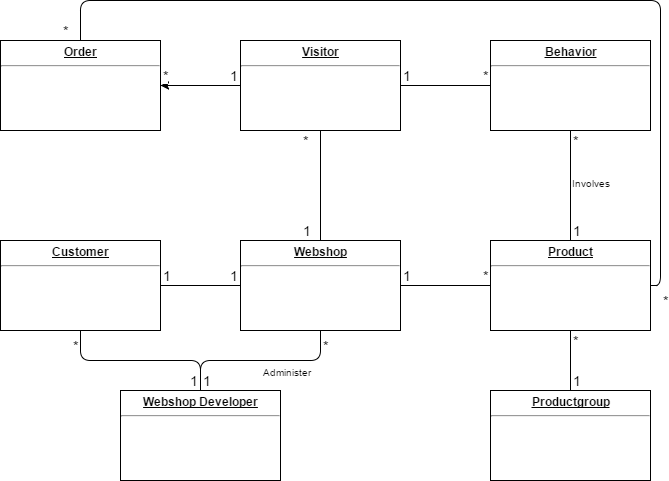
\includegraphics[width=.8\linewidth]{Figures/Domain_model.png}
	\caption{Domain model}
	\label{fig:DomainModel}
\end{figure}

The domain model in figure \ref{fig:DomainModel} is the result of the analysis of the requirements. The domain model provides an overview of concepts in the system, and how they are related.

\begin{description}
	\item[Webshop Developer] is the company developing and hosting a collection of webshops. In this project the \textit{Webshop Developer} is the company Struct A/S, who wish to add value to their services by offering product recommendations. Seen from the perspective of the project group, this is the customer who ordered a recommendation system.
	\item[Customer] is an owner of a \textit{Webshop}, developed by the \textit{Webshop Developer}. \textit{Customer} is a secondary stakeholder that desires the possibility of presenting product recommendations to its visitors.
	\item[Webshop] is the webshop owned by a \textit{Customer}, and developed and hosted by the \textit{Webshop Developer}. \textit{Webshop} offers a variety of products and presents them to the visitors of the site.
	\item[Visitor] is the end-user of the \textit{Webshop}. This is a potential customer to the owner of the \textit{Webshop} and will have product recommendations presented once the recommendation system is applied.
	\item[Product] is the different products available for purchase on the \textit{Webshop}. 
	\item[Productgroup] is the distinction between groups of products.
	\item[Behavior] describes an action of \textit{Visitor} on the \textit{Webshop}. If a \textit{Visitor} clicks on a \textit{Product}, this is considered a \textit{Behavior}. 
\end{description}

\section{API}
The API is essential for making the product recommendation system available to the \textit{Webshop Developer}. The following calls to the API were identified from analyzing the requirements:

\begin{description}
	\item[GetProductRecommendations] allows the client to ask for product recommendations to a \textit{Visitor}.
	\item[StoreBehavior] stores new \textit{Behavior} in the system.
	\item[DeleteBehavior] deletes existing \textit{Behavior} from the system.
	\item[StoreVisitor] stores a new \textit{Visitor} in the system.
	\item[UpdateVisitor] updates information about an existing \textit{Visitor} in the system.
	\item[DeleteVisitor] deletes an existing \textit{Visitor} from the system.
	\item[StoreProduct] stores a new \textit{Product} in the system.
	\item[UpdateProduct] updates information about an existing \textit{Product} in the system.
	\item[DeleteProduct] deletes an existing \textit{Product} from the system.
	\item[StoreOrder] stores a new \textit{Order} in the system.
	\item[DeleteOrder] deletes an existing \textit{Order} from the system.
\end{description}

The discovered API calls indicates that the system will consist of two aspects, data management and product recommendations.\\
Combining the domain model and the API calls grants an overview of the concepts and their relations within the system. 
%!TEX root=../main.tex
% Chapter Template

\chapter{Design} % Main chapter title

\label{Chapter3} % Change X to a consecutive number; for referencing this chapter elsewhere, use \ref{ChapterX}

%----------------------------------------------------------------------------------------
%	SECTION 1
%----------------------------------------------------------------------------------------

\section{Conceptual overview of the system}
The system is developed as a part of the classic architectural pattern, Model-View-Controller (MVC) \ref{PatternsOfEnterprise}. The system itself consists of the Model and Controller part, and lets the client be responsible for the view, which in this case is the web shop. Figure \ref{fig:MVC} shows how the system is layered. Data is sent to the controller which simply communicates the data between the logic (model) of the system and the view. The logic (model) is responsible for communication with the database, calculations regarding product recommendations, and handling new incoming data. The persistance layer is part of the model as described in \cite{PatternsOfEnterprise}  \textit{"When you're working with a model you are thinking about business policies, perhaps database interactions."}.

\begin{figure}[H]
	\centering
	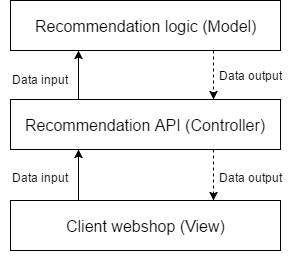
\includegraphics[width=.4\linewidth]{Figures/MVC.png}
	\caption{The Model-View-Controller (MVC) pattern applied on the system}
	\label{fig:MVC}
\end{figure}

\subsection{Recommendation API (Controller)}
The recommendation system is designed according to the MVC pattern described above. The controller layer takes input from the user (the web shop) and passes the information to the model layer. The model layer consists of the objects seen in the domain model in Chapter \ref{analysis} as well as classes for handling the business logic and persistence. The different layers communicate through interfaces in order to be able to substitute implementations in the future. \\
The controller layer is split into two classes, one for handling when the user requests recommendations which relates to functional requirement NF01 and another for handling the data coming from the web shops relating to functional requirements F02-F15.


\subsection{Recommendation logic (Model)}
The recommendation logic is where the main operations of the system takes place. The model layer consists of five packages, and is made accessible to the controller layer through three interfaces. All classes used for calculations are placed in the Business package. This is where the product recommendations are calculated before being sent back to the control layer. This is also the package where any offline-calculation is made before it is stored in the database. The persistence package handles all information that needs to be communicated with the database. The Entities and Utility package creates an easier and more manageable way of communicating data around within the model layer. All communication between the Controller-layer and the Model-layer is done through the interfaces seen in the Communication package. These interfaces are implemented by their corresponding classes in the Business and Persistence packages. The implementation of the Model-layer is discussed further in Chapter \ref{Chapter5}. \\
A package diagram of the Controller and Model layer can be seen in figure \ref{fig:PackageDiagram}

\begin{figure}[H]
	\centering
	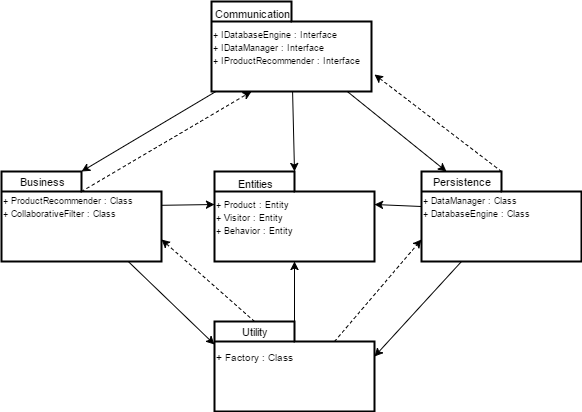
\includegraphics[width=.8\linewidth]{Figures/PackageDiagram.png}
	\caption{Package diagram of the model layer}
	\label{fig:PackageDiagram}
\end{figure}

\section{Client-Server}
When put to use, the recommendation system will be distributed and play the server role in a Client-Server model. The system should be considered an application solely for providing product recommendations. In this scenario, the client is the web shop that needs to provide recommendations to one of its users. The client is also able to ask the server to update its database or store new content in the database, but the concept is the same and just as simple as the request for product recommendations. The Client-Server model of the system can be seen in figure \ref{fig:ClientServer}

\begin{figure}[H]
	\centering
	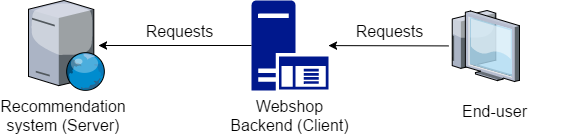
\includegraphics[width=.8\linewidth]{Figures/ClientServer.png}
	\caption{Package diagram of the model layer}
	\label{fig:ClientServer}
\end{figure}

\section{Database design}
Specific requirements for the storage of data was set by Struct, as they wanted a largely scalable structure of the data. The technology chosen was \gls{NoSQL}.
The data demands are not clearly specified in the beginning and with No-SQL it is easy to add or remove data or even change the data types on the fly whereas traditional relational databases have very strict data requirements, this also means that all data restrictions have to be handled in the code. No-SQL's denormalized format also allows for faster retrieval of a single item without having to do joins or complex SQL queries. Finally No-SQL is easier to scale across multiple servers and many engines have built in scaling functionalities \cite{SQLvsNOSQL} which can come in handy when multiple clients begin using the service. A downside of No-SQL compared to relational databases is the fact it does not focus much on Online Transaction Processing (OLTP) which means there is no guarantee that the data is always stored completely. Overall No-SQL is a good fit for this project since scalability and speed is imperative. \\\\

A brief overview of the different terminology for SQL and No-SQL is given in table \ref{sqlvsnosql_table}.
\begin{table}[H]
	\centering
	\caption{SQL vs No-SQL terminology}
	\label{sqlvsnosql_table}
	\begin{tabular}{|l|l|p{8cm}|}
		\hline
		\textbf{SQL}   & \textbf{No-SQL}     & \textbf{Comment}                                                                                                    \\ \hline
		Table & Collection &                                                                                                            \\ \hline
		Row   & Document   & A No-SQL document can contain more complex datatypes compared to a row in SQL e.g arrays or other documents \\
		\hline
	\end{tabular}
\end{table}

The database design mimics the domain model by representing real world concepts such as a Visitors and their Behavior and Products. The No-SQL design can be seen in figure \ref{documents}.

\begin{table}[H]
	\centering
	\caption{An overview of the fields in each document in the collections}
	\label{documents}
	\begin{tabular}{|l|l|p{7cm}|}
		\hline
		\textbf{Document} & \textbf{Fields}                                                                                                                          & \textbf{Comment}                                                                   \\ \hline
		Visitor           & \begin{tabular}[c]{@{}l@{}}Id: string\\ Behaviors: array\\ ProfileUID: string\\ CustomerUID: string\end{tabular}                         & The behavior array is an array of Behavior documents which contains all the behaviors of the specific visitor \\ \hline
		Product           & \begin{tabular}[c]{@{}l@{}}Id: int\\ ProductGroupId: int\\ VisitorId: stringArray\\ Description: string\\ Created: DateTime\end{tabular} &     The visitorId array contains Ids of all visitors who have looked at this product    \\ \hline
		Behavior & \begin{tabular}[c]{@{}l@{}}Type: string \\ Id: int \\ Timestamp: DateTime \end{tabular} & A behavior document holds information about a particular behavior \\ \hline
	\end{tabular}
\end{table}

An example of a Visitort document can be seen in figure \ref{visitorDoc} and an example of a Product document can be seen in appendix \ref{productDoc}.
\begin{figure}[H]
	\centering
	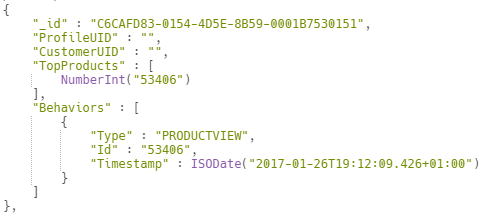
\includegraphics{visitorDocument}
	\caption{A Visitor document example}
	\label{visitorDoc}
\end{figure}

The topProducts array seen in Appendix \ref{productDoc} was not part of the original data transformation, but rather a part of the recommendation algorithm explained in Chapter \ref{Chapter5}.

%!TEX root=../main.tex
% Chapter Template

\chapter{Implementation} % Main chapter title

\label{Chapter5} % Change X to a consecutive number; for referencing this chapter elsewhere, use \ref{ChapterX}

%----------------------------------------------------------------------------------------
%	SECTION 1
%----------------------------------------------------------------------------------------

\section{Solution overview}

The final solution consists of a \gls{REST} API build with ASP.NET Core and a MongoDB \gls{NoSQL} database. Both are hosted through Amazon Webservices in an EC2 container using Docker. \\
The API consists of the commands seen in appendix \ref{APICommands}. \\\\

This section covers the process from the initial data delivery to the final solution in a chronological order.

\section{Initial data dump}
In the beginning of the project we were supplied with data from one of \gls{Struct} customers. This data was in the form of many SQL tables and most of the data was not relevant for creating product recommendations. The main tables used were the following:  \\
\begin{itemize}
\item Visitor: A collection of every unique visitor who visited the customer's website, each visitor gets a unique identifier called UID. Contains 3,073,665  visitors.
\item Profile: A collection of every users signed up at the website. Contains 3037 profiles.
\item BehaviorData: A collection of every unique action performed by visitors on the website, for example when a visitor views a product a new row is made with the visitor's UID, the product UID and the timestamp. Contains 3,326,736 visitor actions.
\item Order: Contains each profile's orders. Contains 5520 orders.
\item Product: A collection of all products on the website with their unique IDs. Contains 22,445 products.
\item ProductGroup: A collection of all product groups. Contains 262 product groups.
\item AttributeValueRendered: A collection of product and product group descriptions in different languages. Contains 409,259 descriptions:

\end{itemize}

A snapshot of the visitor and behaviorData table can be seen in figure \ref{visitorTable} and \ref{behaviorTable}.

\begin{figure}[H]
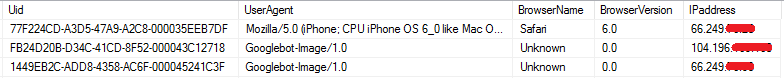
\includegraphics[scale=0.8]{Visitor_table}
\caption{Visitor table from the original data}
\label{visitorTable}
\end{figure}
\begin{figure}[H]
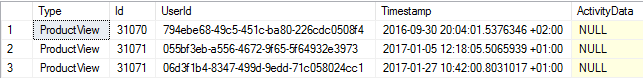
\includegraphics{behaviorData_table}
\caption{Behavior data table from the original data}
\label{behaviorTable}
\end{figure}

These tables contain all the pertinent information for creating product recommendations and can be utilized after a cleaning and structuring process. This process is described in the following sections.

\section{Data Transformation}
To begin the initial data transformation a data storing technology has to be selected. The technology chosen was \gls{NoSQL}, specifically \gls{MongoDB} the most popular No-SQL framework \cite{DBRankings}. \\
\gls{NoSQL} is chosen because of the good fit for this project. The data demands are not clearly specified in the beginning and with No-SQL it is easy to add or remove data or even change the data types on the fly. No-SQL's denormalized format also allows for faster retrieval of a single item without having to do joins or complex SQL queries. Finally No-SQL is easier to scale across multiple servers and many engines have built in scaling functionalities \cite{SQLvsNOSQL} which can come in handy when multiple clients begin using the service. \\\\

A brief overview of the different terminology for SQL and No-SQL is given in table \ref{sqlvsnosql_table}.
\begin{table}[H]
\centering
\caption{SQL vs No-SQL terminology}
\label{sqlvsnosql_table}
\begin{tabular}{|l|l|p{8cm}|}
\hline
\textbf{SQL}   & \textbf{No-SQL}     & \textbf{Comment}                                                                                                    \\ \hline
Table & Collection &                                                                                                            \\ \hline
Row   & Document   & A No-SQL document can contain more complex datatype compared to a row in SQL e.g arrays or other documents \\
\hline
\end{tabular}
\end{table}

Python was used to accomplish the early migration from SQL tables to MongoDB. Several scripts were created to retrieve the data from the SQL server and transfer it to the MongoDB database in the wanted format. Pseudo code of one of these scripts can be seen in algorithm \ref{alg:product}. \\

%Shoud probably be in an appendix.

\begin{algorithm}
\caption{Product Script}
\label{alg:product}
\begin{algorithmic}[1]
	\State SQLquery = SELECT * FROM struct.Product
	\State  db = MongoDB
	\ForAll{Rows r in SQLquery}
	\State   Product = \{Id: r.id 
	\State	\hspace{1cm}		Description: "" 
	\State	\hspace{1cm}		Created: r.created 
	\State	\hspace{1cm}	visitorID: [] 
	\State \hspace{1cm}	ProductGroupId: 0 \}
	\State db.insert(Product)
	\EndFor
	\\
	\State Description = ""
	\State	firstId = true
	\State previousId = 0
	\State previousGroupId = 0
	\State SQLquery = SELECT * FROM struct.product JOIN struct.attributeValueRendered ON id ORDER BY productId desc
	\ForAll{Rows r in SQLquery}
	\State currentId = r.ProductId
	\State currentGroupId = r.GroupId
	\If{firstId}
	\State previousId = currentId
	\State firstId = false
	\EndIf
	\If{currentId != previousId}
	\State db.update(\{id: previousId\},
	\State \hspace{1cm} \$set: db.description: description
		\State db.update(\{id: previousId\},
	\State \hspace{1cm} \$set: db.ProductGroupId: previousGroupId
	\State description = ""
	\EndIf
	\State description += r.description
	\State previousId = currentId
	\State previousgroupId = currentGroupId
	\EndFor
	\State VisitorIds = []
	\State firstId = true
	\State previousId = 0
	\State SQLquery = SELECT * FROM struct.BehaviorData
	\ForAll{Rows r in SQLquery}
	\State currentId = r.Id
	\If{firstId}
	\State previousId = currentId
	\State firstId = false
	\EndIf
	\If{currentId != previousId}
	\State db.update(\{id: previousId\},
	\State \hspace{1cm} \$set: db.VisitorId: visitorIds
		\State db.update(\{id: previousId\},
	\State visitorIds= []
	\EndIf
	\State visitorIds.append(r.UserId)
	\State previousId = currentId
	\EndFor
\end{algorithmic}
\end{algorithm}

After all the scripts are finished the No-SQL database has the collections Visitor and Product. A breakdown of documents in the two collections can be seen in table \ref{documents}	

\begin{table}[H]
\centering
\caption{An overview of the fields in each document in the collections}
\label{documents}
\begin{tabular}{|l|l|p{7cm}|}
\hline
\textbf{Document} & \textbf{Fields}                                                                                                                          & \textbf{Comment}                                                                   \\ \hline
Visitor           & \begin{tabular}[c]{@{}l@{}}Id: string\\ Behaviors: array\\ ProfileUID: string\\ CustomerUID: string\end{tabular}                         & The behavior array is an array of documents with the fields Type, Id and Timestamp. This contains all the behaviors of the specific visitor \\ \hline
Product           & \begin{tabular}[c]{@{}l@{}}Id: int\\ ProductGroupId: int\\ VisitorId: stringArray\\ Description: string\\ Created: DateTime\end{tabular} &     The visitorId array contains Ids of all visitors who have looked at this product    \\ \hline
\end{tabular}
\end{table}

After the data has been cleaned and structured in No-SQL the algorithm for determining product recommendations can be made. The algorithm is described in the following section.

\section{The product recommendation algorithm}
There are multiple ways to implement af product recommendation algorithm all with their advantages and disadvantages. The method chosen for this project is called Item-to-Item collaborative filtering. Other methods and the reasoning why these weren't chosen is described in further detail in Chapter 6 discussion. \\\\

Item-to-Item collaborative filtering is a datamining tool to link items (products) with other items in terms of their similarity. This method is also the way \gls{Amazon} handles their product recommendations \cite{AmazonRecommendations}. \\
The specifics of the algorithm differs from implementation to implementation. In this version each product is compared to other products based on how much they have been viewed together by customers, the likeness of their description and their product group. \\
The first run of the algorithm requires going through each product and the visitors of each product to see what else they have looked at. This needs a lot of resources, but once run only new behavior has to be re-calculated. A run down of the algorithm can be seen in algorithm \ref{alg:collaborativeFilter}. \\\\

\begin{algorithm}[H]
\caption{Item-to-Item collaborative filtering algorithm}
\label{alg:collaborativeFilter}
\begin{algorithmic}[!H]
\ForAll{Products p}
\State productScores = Dictionary<int, double>
\ForAll{Visitors in p}
\ForAll{Products visitorProduct in Visitor behaviors}
\If{productScores contains visitorProduct}
\State productScores[visitorProduct]++
\Else
\State productScores.Add(visitorProduct, 1)
\EndIf
\EndFor
\EndFor
\State Sort productScores after highest value
\ForAll{Products similarProduct in productScores}
\State productScores[similarProduct] = \textbf{calculateSimilarityScore(p, similarProduct, productScores[similarProduct])} (see algorithm \ref{alg:calculateSimilarity})
\EndFor
\State Sort productScores after highest value
\State Store top 10 productScores in database under p
\EndFor
\end{algorithmic}
\end{algorithm}

\begin{algorithm}[H]
\caption{Similarity calculations for two products }
\label{alg:calculateSimilarity}
\begin{algorithmic}[!H]

\State \textbf{calculateSimilarityScore(mainProduct p1, compareProduct p2, currentScore)}
\State similarAttributeFactor = 0.02
\State productGroupFactor = 0
\State numOfSimAttributes = 0
\If{p1.productGroup equals p2.productGroup}
\State productGroupFactor = 0.02
\EndIf
\ForAll{words w in p1.description}
\If{w is in p2.description}
\State numOfSimAttributes++
\EndIf
\EndFor
\If{numOfSimAttributes equals 0}
\State similarAttributeFactor = 0
\EndIf
\State \textbf{return} \begin{math} currentScore * (1+productGroupFactor)*(1+similarAttributeFactor^{numOfSimAttributes}) \end{math}
\end{algorithmic}
\end{algorithm}


After algorithms \ref{alg:collaborativeFilter} and \ref{alg:calculateSimilarity} each product in the database now has an array with the top 10 similar products based on amount of views, description and product group. \\
Next up is calculating the top products for each visitor, these are the products the specific visitor has viewed the most. This is accomplished by iterating through each visitor, checking their behavior and storing their top products as a field in the database. This calculation can be seen in algorithm \ref{alg:topProducts}. This calculation also requires a large amount of resources the first time, but very little to maintain.

\begin{algorithm}[H]
\caption{Calculations of each visitors top products}
\label{alg:topProducts}
\begin{algorithmic}[H]
\ForAll{Visitors v}
\State visitorProducts = Dictionary<string, int>
\ForAll{Behaviors b in v}
\State topVistorProducts[b.Id]++
\EndFor
\State Sort visitorProducts after highest value
\State Store top 5 visitorProducts in database under v
\EndFor
\end{algorithmic}
\end{algorithm}

Since all these calculations are made before the actual product recommendations are requested, the process of recommending products is quite fast. The recommendation process starts with retrieving the requested visitor's top products from the database, retrieving these products top similar products, sorting them based on their score and finally returning the amount asked for. The code for the recommendation part can be seen in algorithm \ref{alg:recommendation}

\begin{algorithm}[H]
\caption{Get product recommendations}
\label{alg:recommendation}
\begin{algorithmic}[H]
\State visitorTopProducts = db.GetTopProducts(visitorUID)
\State productRecommendations = Dictionary<int, double>
\ForAll{Products p in visitorTopProducts}
\State SimilarProducts = db.GetTopProductRecommendation(product)
\ForAll{products simProduct in similarProducts}
\If{productRecommendations contains simProduct}
\State productRecommendations[simProduct] += similarProducts[simProduct]
\Else
\State productRecommendations.add(simProduct, similarProducts[simProduct]
\EndIf
\EndFor
\EndFor
\State Sort productRecommendations after highest value
\State \textbf{return} amount of productRecommendations requested
\State 
\end{algorithmic}
\end{algorithm}

The entire process of requesting product recommendation, running algorithm \ref{alg:recommendation} and returning them takes less than 40ms which is one of the non-functional requirements. \\\\
Some other paths are required in certain situations such as when the visitor does not have any behavior or not enough behavior to satisfy the amount of recommendations requested. In these cases the remaining recommendations are filled from the top 20 most popular products in the last 30 days. The top 20 products are calculated by checking the timestamp and finding those in the last 30 days and then counting how many times each product was viewed. The top 20 products are stored in the database and can be calculated through an API call.

\section{Hosting the API}
An API can be hosted in several different ways, through many providers. This product recommendation API is hosted through Amazon WebServices in an \gls{EC2Instance} \cite{EC2}. To accomplish this the ASP.NET core project is built in a Docker container, the container is pushed to the Docker Hub and then pulled and run in the \gls{EC2Instance}. The database is similarly packed in a docker container and run in the \gls{EC2Instance}. The Docker containers have exposed ports to the rest of the internet and can be accessed via \gls{EC2Instance} public DNS or IP.



			


 
%!TEX root=../main.tex
% Chapter Template

\chapter{Experimental Validation} % Main chapter title

\label{Validation} % Change X to a consecutive number; for referencing this chapter elsewhere, use \ref{ChapterX}

%----------------------------------------------------------------------------------------
%	SECTION 1
%----------------------------------------------------------------------------------------

This section takes a look at the validation of the system from different viewpoints. A validation of the code is described in terms of integration tests. The recommendations are validated statistically by using two standard measures. Concrete examples of recommendations are given to provide some insight into what kind of recommendations are provided for different visitors.

\section{Integration tests}
The code is validated through a series of top-down, black-box integration tests. The purpose of these tests is to ensure the functionality of the two controllers, \textit{ProductRecommendationController} and \textit{DataController}. An overview of the test cases can be seen in table \ref{testCases}.

\begin{table}[H]
\centering
\caption{Integration test cases}
\label{testCases}
\begin{tabular}{|p{6cm}|p{5cm}|p{5cm}|}
\hline
\textbf{Method}             & \textbf{Test Case}                                             & \textbf{Expected Result}           \\ \hline
GetRecommendationForVisitor & Valid arguments                                                & String array of size 5             \\ \hline
GetRecommendationForVisitor & Non existing visitor                                           & String array of size 5             \\ \hline
GetRecommendationForVisitor & Uppercase/lowercase visitorUID                                 & String array of size 5             \\ \hline
GetRecommendationForVisitor & Uppercase/lowercase database                                   & String array of size 5             \\ \hline
GetRecommendationForVisitor & Number of recommendations being larger than available products & String array of all valid products \\ \hline
GetRecommendationForVisitor & Visitor with no behavior                                       & String array of size 5             \\ \hline
GetRecommendationForVisitor & Non existing database                                          & Empty string array                 \\ \hline
PutVisitor                  & New visitor                                                    & HTTP status code 201 created         \\ \hline
PutVisitor                  & Existing visitor                                               & HTTP status code 400 Bad Request            \\ \hline
PutVisitor                  & Non existing database                                          & HTTP status code 400 Bad Request            \\ \hline
PutProduct                  & New product                                                    & HTTP status code 201 created         \\ \hline
PutProduct                  & Existing product                                               & HTTP status code 400 Bad Request            \\ \hline
PutProduct                  & Non existing database                                          & HTTP status code 400 Bad Request           \\ \hline
PutBehavior                 & New behavior                                                   & HTTP status code 200 OK         \\ \hline
PutBehavior                 & Non existing database                                          & HTTP status code 400 Bad Request          \\ \hline
\end{tabular}
\end{table}

Most of the tests of the recommendation part is tested with 5 recommendations being requested, hence the return of a string array with size 5. \\
The put methods should return \textit{HTTP status code 201 Created} if a new item is created in the database, \textit{200 OK} if an item is updated, and \textit{400 Bad Request} if it fails.
All tests run successfully and a result overview can be seen in figure \ref{testResult}
\begin{figure}[H]
\centering
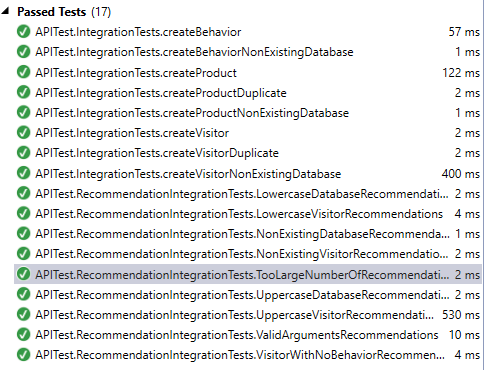
\includegraphics[scale=0.8]{testResults}
\caption{Result of all integration tests}
\label{testResult}
\end{figure}


\section{Validation of recommendations}

Validation of product recommendation engines is focused around two approaches \cite{eval}:
\begin{itemize}
	\item Offline validation
	\item Online validation
\end{itemize}


\subsection{Offline validation}
This section takes two approaches to validating the implemented recommendation engine:
\begin{itemize}
	\item A statistical approach using recall and precision
	\item Concrete examples
\end{itemize}

\subsubsection{Statistical approach}
Recall and Precision are two measures used for offline validation of product recommendation systems. Recall is defined as the number of relevant items (successful guesses) retrieved divided by the total number of relevant items (all behavior). Precision is defined as the number of relevant items retrieved divided by the total number of documents retrieved (all recommendations). \\ In recommendation systems the two measures are also described as follows: 
\begin{description}
	\item [Recall] \textit{a perfect recall score of 1.0 means that all good recommended items were suggested in the list (although says nothing about how many bad recommendations were also in the list)} \cite{recallAndPrecision}
	\item [Precision] \textit{a perfect precision score of 1.0 means that every item recommended in the list was good (although says nothing about if all good recommendations were suggested)} \cite{recallAndPrecision}
\end{description}

These measures are found using a method where a percentage of the data available is used as regular input data and another percentage as test data \cite{eval}. The evaluation run in this project used 80 percent of the data as input and tested on the remaining 20 percent. More specifically the remaining 20 percent was used in the following way:
\begin{itemize}
\item Take each visitor with more than two behaviors
\item Input half of the visitor's behaviors via the API
\item Generate 5 recommendations for the specific visitor
\item See if the remaining half of his behaviors are in the recommended 5 items.
\end{itemize}
The selected 20\% visitors are chosen randomly as they are sorted by Id which is a randomized string assigned to each visitor.

This resulted in a total of 1,934 visitors tested and a total of 9670 recommendations. These visitors have 11,328 behaviors where half was used as input and half was used as control. This means the recommendation engine had to predict half of 11,328 (5,664) behaviors. The algorithm succeeded in correctly predicting 2974 behaviors.  \\
The recall percentage is calculated as \begin{math}2974/5664*100=52.5\%\end{math}. \\ The precision percentage is calculated as \begin{math}2974/9670*100=30.8\%\end{math}. \\
The Recall and Precision rates are visualized in figure \ref{recallAccuracy}. The result of this evaluation as well as the scripts used can be found attached with the source code. \\
\begin{figure}[H]
\centering
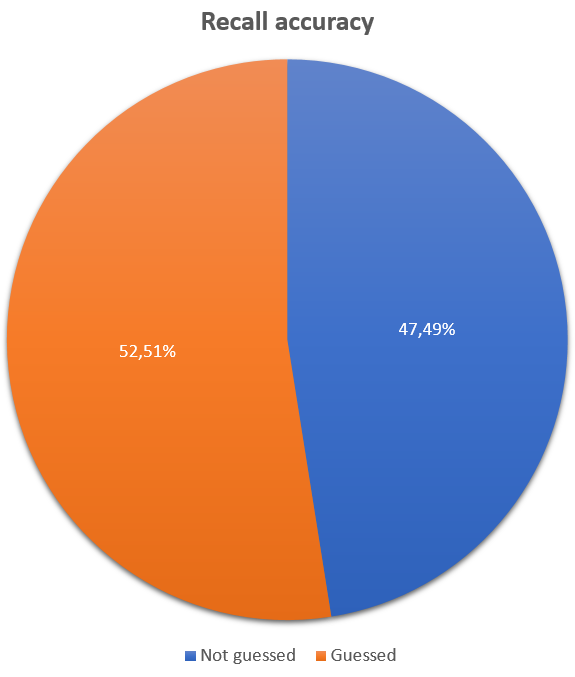
\includegraphics[scale=0.7]{recallAccuracy}
\caption{Recall accuracy}
\label{recallAccuracy}
\end{figure}
The engine only had half of each visitors behavior as input which could be as low as 1 behavior and still managed to guess correctly more than half of the time.
The precision score is only 30.8\% in this test which implies that the algorithm also provides many poor recommendations. One of the major drawbacks of these statistics is the fact that it assumes that every recommended item not in the visitors real behavior is a bad recommendation. This is not always the case as a visitor might not have looked at the product because he was unaware of its existence but might have decided to look at it if it was recommended \cite{evaluatingRecommender}. Another drawback is that the numbers tell nothing about catalog coverage which is how much of the product catalog the recommendation system recommends. It is therefore possible to have a good recall rate but not be suggesting anything new to the visitors \cite{eval}.
As the algorithm acquires more data on all visitors the precision should increase.\\
Root-Mean-Square-Error (RMSE) and Mean-Absolute-Error (MAE) \cite{rmseAndmae} are other measures used in offline validation. These measures require user ratings on products which is not present in the data for this project. RMSE and MAE can therefore not be used to evaluate these product recommendations. \\
\subsubsection{Concrete examples}
To give a better understanding of the recommendations given by the algorithm a few specific examples are given below. \\

\textbf{Visitor A} has looked at the following products:
\begin{itemize}
\item \textbf{36991: }Playset Brandmand Sam fyrtårn med figur
\item \textbf{37691: }Playset Brandmand Sam Havnestation
\item \textbf{37799: }Firman Sam Ocean Rescue
\item \textbf{38950: }Sejt Brandmand Sam udstyrssæt
\item \textbf{40786: }Brandmand Sam helikopter med lys og lyd
\item \textbf{42373: }Biler Brandmand Sam og brandbil
\item \textbf{52818: }Udklædning tilbehør sej Brandmand Sam megafon
\item \textbf{52919: }Playset Fireman Sam
\end{itemize}
and is recommended the following products:
\begin{itemize}
\item \textbf{43215: }Biler Brandmand Sam bil
\item \textbf{36991: }Payset Brandmand Sam fyrtårn med figur
\item \textbf{37799: }Firman Sam Ocean Rescue
\item \textbf{38950: }Sejt Brandmand Sam udstyrssæt med bælte
\item \textbf{34392:} Brandmand Sam 104 cm Fastelavnstøj
\end{itemize}

The visitor has already looked at some of the recommended items. As the recommendations size increases more new products to the visitor will appear. The recommendations are all "Brandmand Sam" products which is all he has looked at in the past. Whether it is good or bad depends on the business and how the visitors will respond. These recommendations are in accordance with the wishes of \gls{Struct} as they want very similar items to be recommended. Presenting the same products to a user several times can also increase the likelihood of a purchase happening. In the future the recommendation engine will be able to filter already purchased products, but this has yet to be implemented. \\\\

Another \textbf{visitor B} has looked at the following products:
\begin{itemize}
\item \textbf{43106: }Biler Scalextric C3528 BMW MINI Cooper S
\item \textbf{49777: }Scalextric Racerbane C1368 Bilbaner Le Mans Prototypes Sports Cars
\item \textbf{33136: }Chevrolet Camaro GT-R Biler Scalextric C3383 
\item \textbf{43104: }Scalextric C3524 VW Polo WRC Biler
\end{itemize}
and is recommended the following 5 products:
\begin{itemize}
\item \textbf{43106: }Biler Scalextric C3528 BMW MINI Cooper S
\item \textbf{43104: }Scalextric C3524 VW Polo WRC Biler
\item \textbf{49777: }Scalextric Racerbane C1368 Bilbaner Le Mans Prototypes Sports Cars
\item \textbf{33136: }Chevrolet Camaro GT-R Biler Scalextric C3383
\item \textbf{42841: }Maserati Trofeo Biler Scalextric C3388
\end{itemize}

These recommendations also relate closely to the products the visitor has viewed. \\\\

A final example \textbf{visitor C} has looked at these products:
\begin{itemize}
\item \textbf{42809: }Bosch arbejdsbord Bosch Værktøj og Værktøjsbænke
\item \textbf{42106: }Elsker du også bare paw patrol
\end{itemize}
and is recommended these products:
\begin{itemize}
\item \textbf{42106: }Elsker du også bare paw patrol
\item \textbf{42809: }Bosch arbejdsbord Bosch Værktøj og Værktøjsbænke
\item \textbf{40542: }LEGO Legends Of Chima Flyv op gennem skyerne
\item \textbf{31548:} LEGO Legends Of Chima Snurrende slyngplanter
\item \textbf{43713:} Fastelavnstøj Tid til at ringe efter politiet og Paw Patrols hund nummer 1
\end{itemize}
The two LEGO recommendations in this example might not seem thematically accurate, however since they have been recommended they must have a high similarity score to one or both of the products the visitor has looked at. A closer look at the data shows the two LEGO products to have similarity scores of 24 and 15 respectively to product 42106. Since these products are not in the same product group and have zero matching descriptions the high similarity score is the amount of times they have been looked at together with this product. The main product, product 42106, have been looked at by 9 other visitors and these 9 visitors have looked at the first LEGO product 24 times and the second LEGO product 15 times.

\subsection{Online validation}
When the recommendation algorithm is put into production, several new and better ways of evaluating the system becomes available. As the visitors get recommendations their behavior is logged and it is possible to see how many of the recommendations are actually used and adjust the algorithm thereafter. Online validations have not been possible as part of the project scope. In an online scenario the recommendations could be examined by calculating click-through rates and conversion rate. Click-through rate is how many percent of the recommendations have resulted in the visitor viewing the product. Conversion rate is how many percent of the recommendations have resulted in a purchase. Furthermore the turnover of the web shop can be analyzed over a period of time to measure whether or not the recommendations are effective.
This adjustment can potentially be automated by using machine learning - this is covered in more detail in chapter \ref{Chapter9}.

 
% Chapter Template

\chapter{Discussion} % Main chapter title

\label{Chapter7} % Change X to a consecutive number; for referencing this chapter elsewhere, use \ref{ChapterX}

%----------------------------------------------------------------------------------------
%	SECTION 1
%----------------------------------------------------------------------------------------
\section{Data storage}
The first focus of the project was to organize a lot of data. This was done with the No-SQL framework, MongoDB. No-SQL was chosen because of its great flexibility and its high performance even when the amount of data accumulates. With the amount of data used for datamining, the project might have been a success if a traditional SQL database had been used. However, Struct A/S asked for a scalable way of handling the data was it to exceed billions of records. In order to accommodate this requirement, No-SQL was the better choice.

\section{Maintainability}
Another important issue was to create a system that allowed for easy maintenance. Amazon web-services served as the tool for deploying the system, and Docker created an environment that will make later updates easy to apply. The system itself has been developed in a way that allows each individual client (unique webshop) to feed it with new data. New calculations will automatically be done when new data is stored. This ensures that the recommendation algorithm is always creating recommendations based on the newest information. Other web-services could have been used, but as a low-budget project Amazon offered the best tools for free.
Instead of using docker the application itself could have been deployed on a windows server, and the system would be just as easy accessible. This would have made the deployment part of the project a lot easier, since we would not have to learn a new technology. Using the Docker container allows for cross-platform deployment, and will be easier to deploy elsewhere in the future if needed.

\section{Product recommendations}
The main problem was to develop a good quality product recommendation algorithm. The algorithm of the project did undergo a lot of changing during the process. A user-to-user collaborative filtering algorithm was first implemented, but resulted in slow response times. The clustering method was declined before implementation, because research indicated that this would result in poor recommendations. \cite{AmazonRecommendations} In the end item-to-item collaborative filtering was applied, which meant more datamining and more offline calculations. If the initial research about recommendation technologies had been more thorough, valuable time would not have been wasted on implementing the wrong algorithm. However, the mistakes gave great educational value and the final algorithm was implemented in a short amount of time. Which was due to the understanding gained while developing the initial algorithm.\\
The algorithm is meant to tailor the recommendations to each individual visitor. This is partly succeeded, but the item-to-item collaborative filter is based on the average customer behavior. This could result in poor recommendations for customers with more unique shopping habbits. Furthermore, if a new product is added, it would have to be visited by many different visitors before it would be recommended.

\section{Evaluating the algorithm}
One of the big challenges after implementing the recommendation algorithm was the evaluation. A comparison with Amazon's algorithm would be optimal, but Amazon does not share their algorithm with the public. Even better would be an online evaluation, as mentioned in chapter \ref{Chapter6}. A comparison to other open-source algorithms could be done, but the amount of resources required to setup such an experiment would drift the focus of the project in a wrong direction. The recall method appeared as the best offline option, however did not give the best objective evaluation of the final system. Combining the concrete examples with the recall evaluation did, however, provide a more nuanced justification of the final product.
%!TEX root=../main.tex
% Chapter Template

\chapter{Conclusion} % Main chapter title

\label{Chapter8} % Change X to a consecutive number; for referencing this chapter elsewhere, use \ref{ChapterX}

%----------------------------------------------------------------------------------------
%	SECTION 1
%----------------------------------------------------------------------------------------

\section{Problem definition and research questions}

The original problem definition was supplied by Struct A/S and involves them using their logged user activity data to create a personalized experience for the users. The final solution is an API giving tailored product recommendations to the end users based on their behavior on the website. The API allows for an easy way to add and maintain data about each visitor to keep recommendations up-to-date and relevant. \\
The problem definition derived the following three research questions "How can large amounts of data be optimally organized, stored and accessed in a scalable way?",  "How can this data be maintained and updated easily after deployment?" and How can the organized data be utilized to generate tailored product recommendations for the end user?". These questions are answered below.

\subsection{How can large amounts of data be optimally organized, stored and accessed in a scalable way?}
MongoDB, a No-SQL database, was chosen in order to accomplish scalable accessing and storing of the data provided by Struct A/S. MongoDB provides scaling functionalities due to its denormalized data which can more easily be spread across multiple servers \ref{SQLvsNOSQL}. No-SQL services on platforms such as Azure or Amazon WebServices have built in scaling functions \cite{azureNoSQL} which gives the distinct advantage that even if the data grows exponentially the hardware can keep up. The scaling functionality was not used, due to limited funds. Accessing all information about a certain user or product is simple due to the denormalized structure. Overall MongoDB is a good fit for this type of project with growing data needs.

\subsection{How can this data be maintained and updated easily after deployment?}
Maintaining and updating the data is as simple as calling the API functions as new data is produced. When a new visitor visits the site an API function will store the visitor in the database, similarly new behavior data is stored by calling another API function. These API functions can be called asynchronously meaning no extra load times for the end user, which is important in the online world.

\subsection{How can the organized data be utilized to generate tailored product recommendations for the end user?}
The data can be utilized through datamining. The datamining technique used to generate product recommendations in the project is Item-to-Item collaborative filtering. This process creates links between products based on their similarity and end users can thereby receive product recommendations based on the products they have already looked at. The recommendations are based on the entire user base and assumes users have similar tastes and purchasing patterns.

\section{Requirements fulfillment}
The requirements engineering process created \textbf{15} functional and 4 non-functional requirements. Of these requirements the most important one is F01 which is successfully met. The functional requirements F02, F03, F05 and F06 have also been met. The remaining functional requirements are not met but are not imperative for generating product recommendations. The API is developed in ASP.NET core. The data is stored in a No-SQL database. The API is accessible through the Docker container hosted on Amazon WebServices. Finally the product recommendations are generated in less than 40ms which means all non-functional requirements have been met.

\include{Chapters/Chapter9_futurework}
%\include{Chapters/Chapter5} 
%\include{Chapters/Chapter6}
%\include{Chapters/Chapter7} 
%\include{Chapters/Conclusion}
%\include{Chapters/Chapter8}
%\include{Chapters/Chapter9}
%\include{Chapters/Chapter10}

%----------------------------------------------------------------------------------------
%	THESIS CONTENT - APPENDICES
%----------------------------------------------------------------------------------------

\appendix % Cue to tell LaTeX that the following "chapters" are Appendices
\begin{landscape}
\chapter{API commands} % Main appendix title
\label{APICommands}
\begin{table}[H]
\centering
\begin{adjustbox}{max height=\textheight}
\begin{tabular}{|p{5cm}|p{5cm}|p{5cm}|p{5cm}|}
\hline
\textbf{Function} & \textbf{URI}                                                        & \textbf{Example}                                                         & \textbf{Description}                                                                                                                                \\
\hline
GET      & \seqsplit{recommendation/visitorUID/numberOfRecommendations/database} & \seqsplit{recommendation/AAF995AE-1DD0-41C6-898B-9CBEE884E553/5/Pandashop} & Returns a JSON array of size numberOfRecommendations containing productUIDs which are the product recommendations for the specific visitor \\
\hline
PUT      & \seqsplit{visitor/visitorUID/database} & \seqsplit{visitor/AAF995AE-1DD0-41C6-898B-9CBEE884E553/Pandashop} & Registers a new visitor with the database \\
\hline
PUT      & \seqsplit{product/productUID/description/productGroup/database} & \seqsplit{product/5352/A great product/5/Pandashop} & Registers a new product along with its description and product group with the database \\
\hline
PUT      & \seqsplit{behavior/visitorUID/behaviorType/ItemID/database} & \seqsplit{behavior/AAF995AE-1DD0-41C6-898B-9CBEE884E553/ProductView/5352/Pandashop} & Registers a new behavior for the specific visitor with the database \\
\hline
PUT      & \seqsplit{Update/database/password} & \seqsplit{Update/pandashop/supersecretpassword} & Builds the collaborative filter for the database \\
\hline
PUT      & \seqsplit{Updatevisitortopproducts/database/password} & \seqsplit{Updatevisitortopproducts/pandashop/supersecretpassword} & Updates the top products for all visitors \\
\hline
PUT      & \seqsplit{calculateTop20/database/password} & \seqsplit{calculateTop20/pandashop/supersecretpassword} & calculates the top 20 products in the last 30 days \\
\hline
\end{tabular}
\end{adjustbox}
\end{table}

\end{landscape}
\chapter{Python script for transfering products} % Main appendix title
\label{PythonScript}
\begin{figure}[H]
\centering
\includegraphics[scale=0.9]{pythonalgorithm}
\end{figure}
\chapter{No-SQL Product Document} % Main appendix title
\label{productDoc}
\begin{figure}[H]
\centering
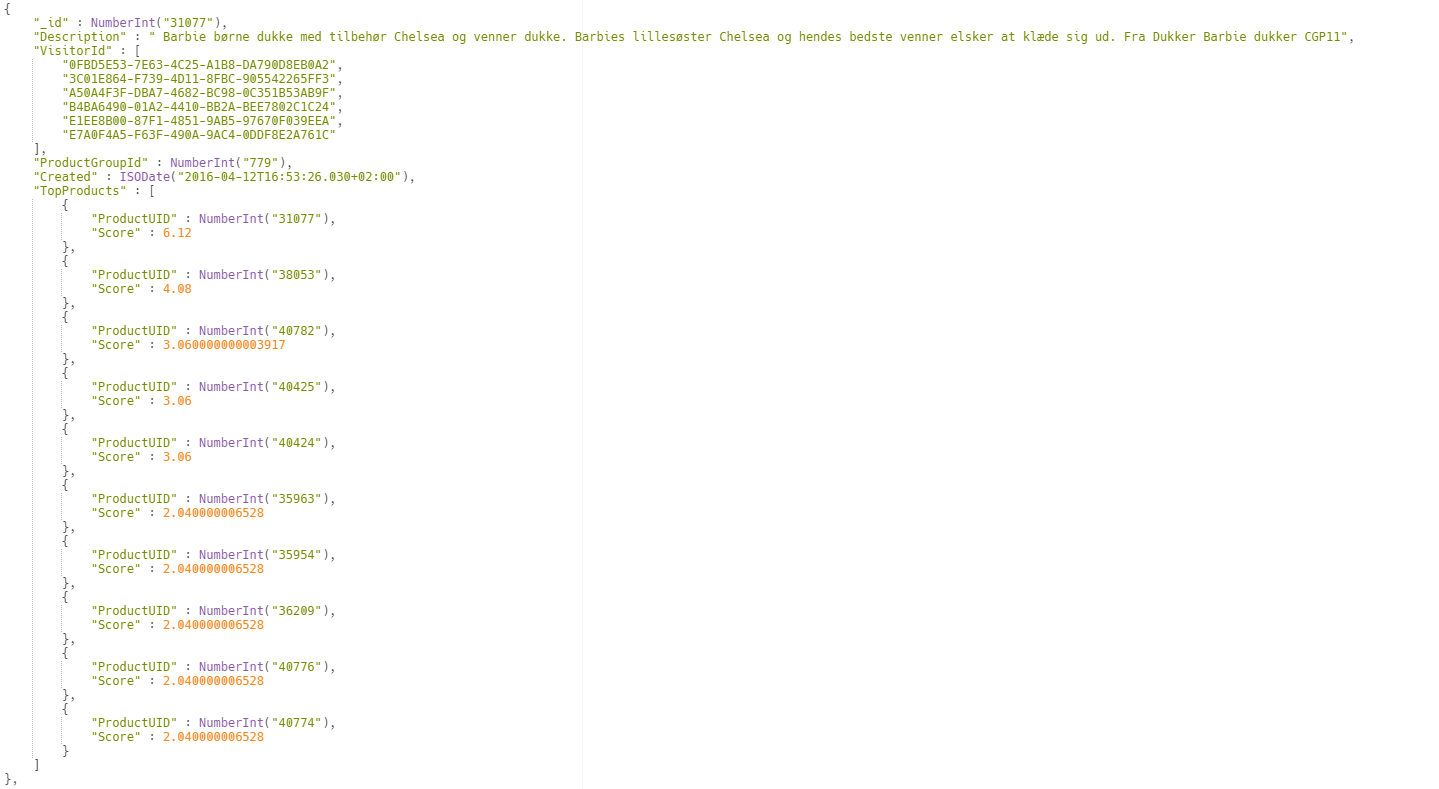
\includegraphics[scale=0.8]{productDocument}
\caption{A Product document example}
\end{figure}
% Chapter Template

\chapter{Process} % Main chapter title

\label{Appendix D} % Change X to a consecutive number; for referencing this chapter elsewhere, use \ref{ChapterX}

%----------------------------------------------------------------------------------------
%	SECTION 1
%----------------------------------------------------------------------------------------

\section{Introduction}
This appendix elaborates on the process behind the development of the final product.

The project was initiated by the case presented by Struct A/S. The core of the case was as follows:
\textit{"When launching sites, whether it being regular websites or web shops, a lot of user activity is logged. We therefore have a large amount of data associated with each of our sites but do not currently use it.} \\
\textit{In the future we would like to be able to use logged data to generate an insight into the user activity on our site and actively use this data to create a personalized experience for the users."} \\
Eventually this case led to the problem statement seen in chapter \ref{Problem}.

A variety of technologies and methods was used throughout the realization of the product. To ensure that the process went as smooth as possible, the agile software development framework, Scrum, was used as a framework to structure and organize the work \cite{Scrum}.

\section{Scrum}
Scrum is the main pillar for controlling the process of the project. Since the developing team only consisted of two students, Scrum is not applied 100\% to the project. This section elaborates on the usage of Scrum and how the different roles were fulfilled.

\subsection{Product owner}
The product owner is typically in charge of which tasks needs to be done in what order. He is in charge of the product backlog and ensures that the developing team keeps adding value to the final product. Since there was no product owner in this project, the role is carried out by the team itself together with the company. The project group kept track of the backlog and had regular feedback from Struct, to ensure the development was on the right track.

\subsection{Scrum master}
The scrum master has the responsibility of removing impediments to the development team, and ensures that the scrum framework is followed. No actual scrum master was elected, which means that the development team along with our supervisor took on the role.

\subsection{Workflow}
Sprints of the length two weeks were chosen, as this was a fitting amount of time to develop and gain feedback. The sprint backlog was filled with issues and prepared before every the start of each sprint. Every work day started with a scrum meeting, where todays work was discussed. At the end of each sprint a meeting was set up with the customer (Struct A/S) to present what was implemented to ensure the project was still on the right track. The sprint backlog for the next iteration was presented as well, and then adjusted according to any feedback from the customer.
By following these two week sprints, the project never deviated much from the wishes of the customer.


\section{GitHub}
The implementation of the final product required the usage of different tools. Github made it possible to structure and organize the planning and implementation of the project.\\

Git is a popular version control system and it is often used when developing software. GitHub is a web-based Git, and served as the primary tool when planning and developing the system. All planning is documented through GitHub issues and milestones. At the initial start, all project tasks was put in the product backlog which was made of issues. The sprints were created as milestones which were filled with issues before each iteration.
The implementation of the system was controlled with Git. A consistent way of using the tool ensured that the newest version of the system was always available to the other group member, and a roleback was always possible had it been necessary. The newest version of the system was always to be found on the \textit{master} branch. When adding new code, the group members had to create a new branch from the \textit{master} branch, to avoid conflicts later. Once the new code was added in its own branch, and tested to ensure there were no flaws, it was merged into the newest version of the \textit{master} branch.
Besides making it possible to work simultaneously on the project, GitHub also served as a backup of the entire project.

\chapter{Case}
\label{Case}
\begin{figure}[H]
	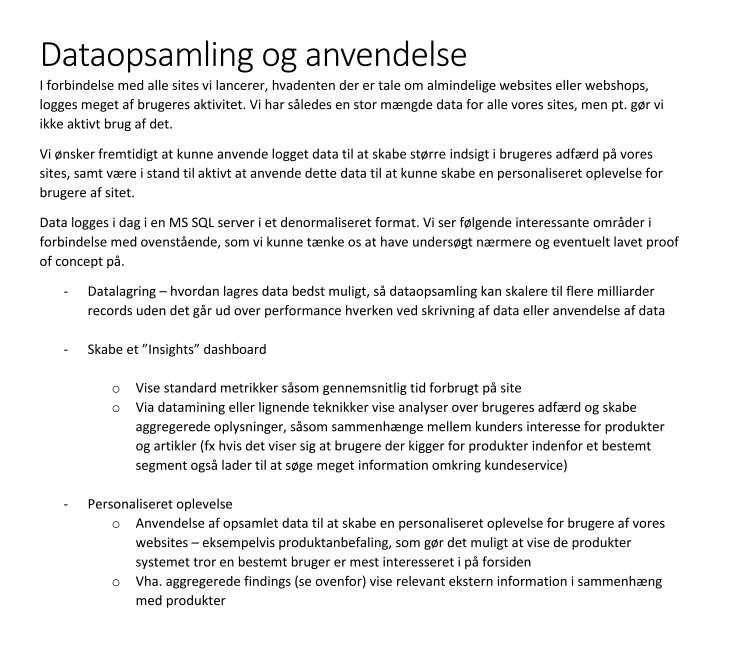
\includegraphics[scale=0.9]{Figures/Case}
	\caption{Original case given by Struct A/S}
\end{figure}
%\input{Appendices/Test-results}
%\input{Appendices/Tidslinje}
% Include the appendices of the thesis as separate files from the Appendices folder
% Uncomment the lines as you write the Appendices

%\include{Appendices/AppendixA}
%\include{Appendices/AppendixB}
%\include{Appendices/AppendixC}

%----------------------------------------------------------------------------------------
%	BIBLIOGRAPHY
%----------------------------------------------------------------------------------------

\printbibliography[heading=bibintoc]

%----------------------------------------------------------------------------------------

\end{document}  
